% !TeX root = ../../main.tex
\section{Experiments}\label{section:experiments}

Three main experiments were implemented to show how the smartphone can help with common interactions when using \ac{VR} software.
To achieve consistency amongst all experiments in terms of look and functionality, a parent class was implemented. The parent class implements multiple utilities and helpers, which are required by each experiment. It also sets up a basic scene, which contains a sky, a floor and lights.  Also the connection to the \ac{UBII} server is handled. 


\subsection{Model Viewer}\label{subsection:model-viewer}

\acf{VR} offers a new way of experiencing \ac{3D} content. It is faster to view a model from different angles and gives a feel of a real presence of the object. Model viewers like Sketchfab\footnote{Sketchfab is an online platform to public and view 3D content. Website: \href{https://sketchfab.com}{www.sketchfab.com}} implemented \ac{VR} support a while ago~\cite{AlbanDenoyel.2016}. But this experience can be enhanced with a smart phone. Models can be rotated without changing the position by walking.

\citeauthor{Katzakis.2010} implemented this without \ac{VR}. His approach uses a smart phone to rotate a model, which is displayed on a conventional display. He uses a similar setup, where the phone is wireless connected to a computer, where the model is rendered. The orientation data comes from the magnetometer and, once calibrated to the screen position, is directly mapped to the model~\cite[139]{Katzakis.2010}. In the comparison against a mouse and a touch pen, the smart phone clearly wins in terms of the time it takes to rotate to a certain pose~\cite[140]{Katzakis.2010}. 
Since this approach turned out to be very successful, it was used in this experiment. 

To feature how easy it is, to view a complex model using VR and the smart phone as a manipulator, a skeleton model is used. This experiment is the only one, supporting more than one smart phone client at the moment. For every client that connects, a new skeleton is created. The position is fixed and arranged around the position of the \ac{VR} headset. The scene is shown in Figure~\ref{fig:screenshot-exp-mv}.

\begin{figure}[htpb]
  \centering
  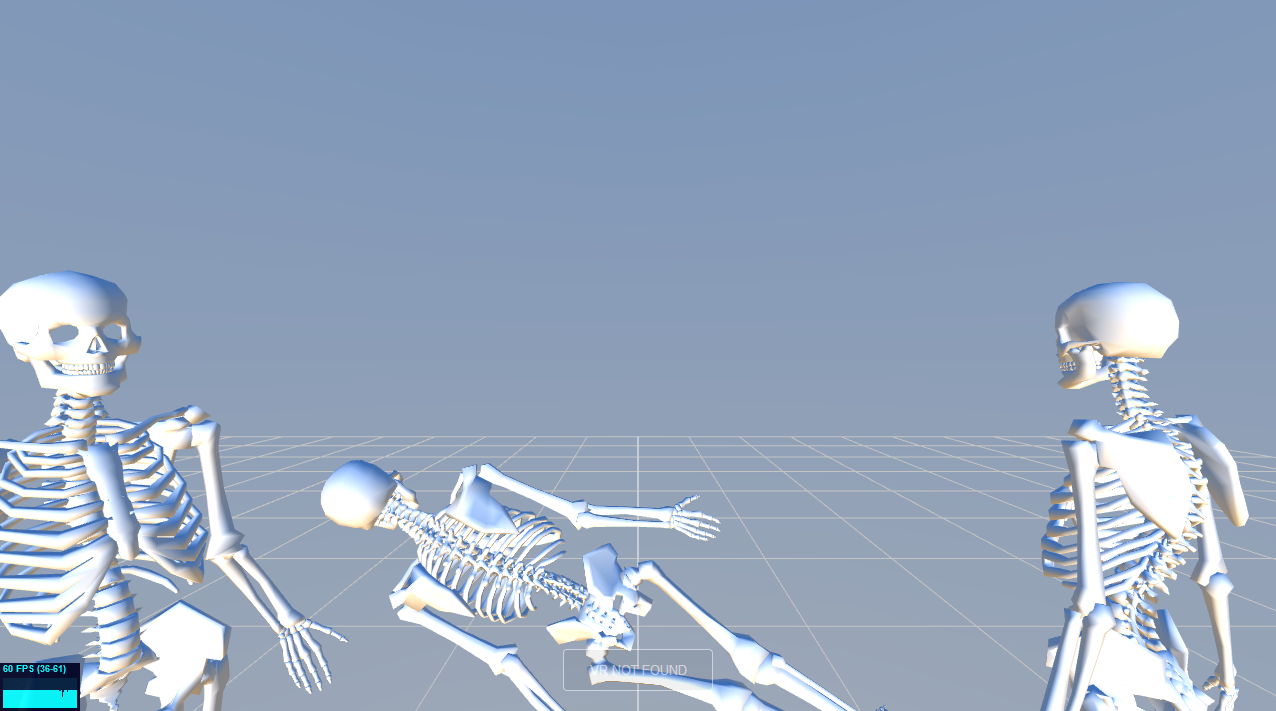
\includegraphics[width=12cm]{figures/screenshot_exp_mv.png}
  \caption[Screenshot: model viewer experiment]{A screenshot of three devices being connected and controlling the rotation of the skeletons.}\label{fig:screenshot-exp-mv}
\end{figure}

% Note: latex thinks the hbox is overfull. This is not the case because something is fixing it. Try removing all words after the lstinline, then you will see that it overflows. But when using in an sentence it appears to be rescaled.
The implentation of this experiment listens for new clients. As soon as one connects, a new interaction is published and the resulting topic subscribed. Since the smart device publishes the orientation data in a different format than ThreeJS needs for rendering, a reusable interaction is created. The interaction converts the angles from radian to degrees, changes the coordinate system and publishes them to the \lstinline{[client id]/web-interface-smart-device/orientation}. The code for the interaction is shown in Figure~\ref{fig:ubii-interaction-angles}.

\begin{figure}[H]
  \begin{lstlisting}[language=JavaScript]
    function (input, output, state) {
      if (!input) {
        return;
      }

      const deg2Rad = function(v) {
        return v * Math.PI / 180;
      };

      output.orientation = {
        x: deg2Rad(input.orientation.y),
        y: deg2Rad(input.orientation.x),
        z: deg2Rad(-input.orientation.z)
      };
    }
  \end{lstlisting}
  \caption[UBII interaction converting euler angles in radians to degrees]{This interaction is used to convert the orientation data sent by the smart device to the format ThreeJS needs for rendering. }\label{fig:ubii-interaction-angles}
\end{figure}